\section{Résultats}

	\subsection{Retour sur les objectifs}
	
		\subsubsection{Protection des modules}
	
			\paragraph{}
			Toutes les protections d'écrite dans le cahier des charges et le cahier de conception ont été implémentées et validées. La précision des différentes mesures répond aux spécifications de la compétition sans même être filtrée numériquement.

		\subsubsection{Balancement des modules}

			\paragraph{}
			L'algorithme et le régulateur pour balancer les modules a été simulé, mais il est impossible pour le moment de le tester. Étant donné que le BMS n'a pas encore passé une batterie de tests exhaustifs, l'équipe a jugé que ce n'était pas sécuritaire d'utiliser un module pour tester la fonctionnalité. Un circuit qui émule le comportement d'une cellule lithium-ion est en cours de fabrication et sera utilisé ultérieurement.
	
		\subsubsection{Compatibilité avec le BMS Lithium Balance}
	
			\paragraph{}
			La carte maître possède le même connecteur que celui utilisé par Lithium Balance avec tous les mêmes périphériques. Les fonctionnalités qui ne sont pas utilisées dans Éclipse IX n'ont pas été programmées.
		
		\subsubsection{Réduction des manipulations lors des vérifications techniques}
	
			\paragraph{}
			Le nombre de manipulations a été réduit en utilisant des mesures différentielles isolées pour les lectures de modules avec un connecteur par lecture. Les thermistances peuvent être facilement remplacées pour la vérification technique. La même stratégie a été utilisé pour la lecture de courant. En ayant une carte séparée et le même connecteur que les autres mesures, il est possible de passer de la résistance de lecture à la composante de test en une manipulation. Les manipulations sont maintenant plus sécuritaires et moins restrictives dans le cas des vérifications pour la surtension et la sous-tension. Ces dernières peuvent maintenant être effectuées sur n'importe quelle cellule contrairement au dernier BMS qui demandait que ce soit tester sur les modules aux deux extrémités.


	\subsection{Tableau des résultats}

		\paragraph{}
		
		\begin{table}[H]
			\centering
			\renewcommand{\arraystretch}{1.3}
			\begin{tabular}{|l|c|c|c|c|}
				\hline
				\textbf{Fonctionnalités} & \textbf{Paramètres} & \textbf{Spécification ciblé} & \textbf{Résultat obtenue} & \textbf{Unité} \\ \hhline{|=|=|=|=|=|}
				\multirow{2}{5cm}{Lecture de tension des modules} & Tension d'entrée & 2 à 5 & 2 à 4.8 & V \\ \hhline{|~|-|-|-|-|}
				& Résolution & 10 & 3 & mV \\ \hline
				\multirow{2}{5cm}{Lecture de courant} & Courant & -22 +130 & $\pm$ 136 & A \\ \hhline{|~|-|-|-|-|}
				& Résolution & $\pm$ 2 & $\pm$ 0.6 & \% \\ \hline
				\multirow{2}{5cm}{Lecture de température} & Région d'opération & -10 à 85 & -40 à 125 & $\degres$C \\ \hhline{|~|-|-|-|-|}
				& Résolution & $\pm$ 2 & $\pm$ 0.2 & \% \\ \hline
				Faciliter les manipulations & Manipulation & 12 & 6 & \\ \hline
				Détection d'une faute & Délais & 200 & 100 & ms \\ \hline
				\multirow{3}{5cm}{Sécuriser la batterie} & Délais & 200 & 100 & ms \\ \hhline{|~|-|-|-|-|}
				& Tension& 0 & 0 & V \\ \hhline{|~|-|-|-|-|}
				& Courant& 0 & 0 & A \\ \hline
				Précharge & Temps & 10 & Théorique : 5.5 & s \\ \hline
				 
			\end{tabular}
		\end{table}
		
	\subsection{Premiers prototypes}
	
		\begin{figure}[H]
			\begin{minipage}{0.45\textwidth}
				\centering
				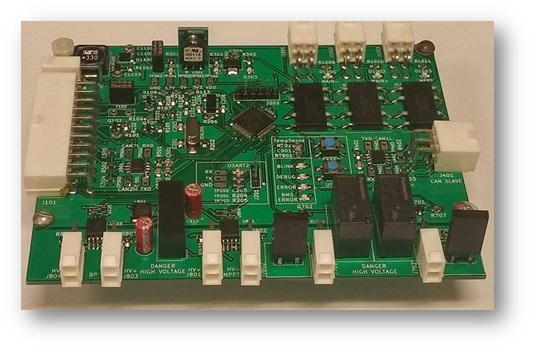
\includegraphics[scale=0.5]{images/master.jpg}
				\caption{Module maître}
				\label{fig:titre1}
			\end{minipage}
			\hfill
			\begin{minipage}{0.45\textwidth}
				\centering
				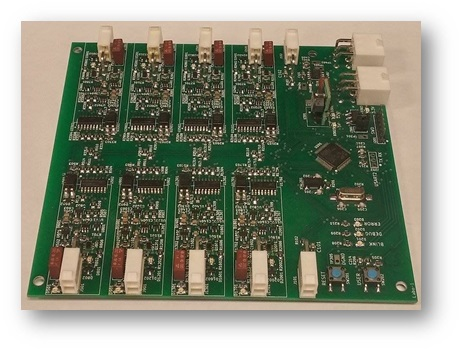
\includegraphics[scale=0.5]{images/slave.jpg}
				\caption{Module esclave}
				\label{fig:titre2}
			\end{minipage}	
		\end{figure}
	
		\begin{figure}[H]
			\centering
			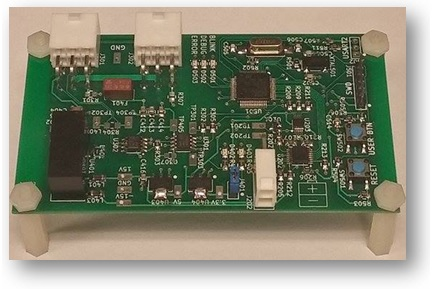
\includegraphics[scale=0.5]{images/currentsense.jpg}
			\caption{Carte de lecture de courant}
			\label{fig:titre3}
		\end{figure}